\chapter {Relationship between orientation tuning and spatial frequency tuning in the tree shrew V1}
\pagebreak
\section{Summary}
\pagebreak
\section{Introduction}

Cortical units selectively respond to edges of a narrow range of orientations unlike their LGN counterparts which respond to almost all orientations. Initial insights into this orientation selectivity, were gained from experiments conducted by Hubel and Wiesel. They proposed a theory of excitatory convergence to explain the sharp orientation tuning they observed in cortical simple cells in cats (Hubel \& Wiesel, 1962) and macaques (Hubel \& Wiesel, 1968). They suggested that un-oriented, spatially offset LGN receptive fields arranged collinearly along the long axis of the cortical receptive field, provided inputs to a simple cell giving rise to the classical, elongated receptive fields and sharp orientation tuning observed in cats and macaques (Hubel \& Wiesel, 1962; 1968).While this has been the most prominent theory of orientation selectivity, still retaining support some 50 years after its conception, it is not without its flaws(for review see Vidyasagar et al., 1996; Ferster \& Miller, 2000). For example, while it explains length summation in the cortical neurons, the excitatory convergence model is unable to account for the contrast invariance observed in simple cells (Ferster \& Miller, 2000; Carandini, 2007).The effectof inhibition generated by intracortical interactions have also been implicated in generating the sharp orientation tuning (Creutzfeldt et al., 1974; Sillito, 1975; 1979; Tsumoto et al., 1979; Sillito et al., 1980). In the light of these short comings, many alternative models of orientation selectivity have been proposed. 

Other models of orientation tuning involve the role of intracortical circuits in the generation of sharp orientation tuning. These models include processes such as cross-orientation inhibition generated by inhibitory interneurons (Creutzfeldt et al., 1974), iso-orientation facilitation (Douglas et al., 1991; Volgushev et al., 1995), spatially offset excitatory and inhibitory inputs (Heggelund, 1981) and excitatory inputs originating from on and off centred neurons (Soodak, 1987). The models that implicate the intracortical circuits also do not take into account of the weak orientation bias reported in the LGN afferents to the cortical cell. The studies that have shown orientation biases in the afferent input to the cortical cell had assumed that this bias originates from a Hubel and Wiesel type excitatory convergence (for example, see Ferster \& Miller, 2000). Soodak's (1987) model ignores the evidence that in studies where APB (suppresses ON responses in bipolar cells) is administered intravitreally in cats, the orientation tuning of the remaining OFF response often stays unchanged in both cats and monkeys (Schiller, 1982, 1986; Sherk \& Horton, 1984; for review see Schiller, 1992).

One model of orientation selectivity suggests that the initial orientation tuning is inherited from the orientation biases of LGN neurons(Vidyasagar et al., 1996). According to this model,the bias in the afferent LGN input to a striate simple cell is established by the excitatory input from one or more LGN receptive fields broadly tuned to the same orientation. In line with this model, orientation biases have been demonstrated in the LGN of cats (Vidyasagar \& Urbas, 1982), macaques (Shou \& Leventhal, 1989) and tree shrews (Van Hooser et al., 2013). Once an initial orientation selectivity is established from the LGN input, recurrent excitation and inhibition caused by the extensive horizontal connections in V1; cross-orientation inhibition and non-specific inhibition may all contribute to sharpen orientation tuning (Vidyasagar et al., 1996).

Sine-wave gratings have been used to study both spatial frequency tuning and orientation tuning in neurons along the visual pathway. When thus examined, cortical cells exhibit band-pass tuning to spatial frequency i.e., they respond to a narrow range of spatial frequencies. Their LGN counterparts on the other hand show a low-pass spatial frequency tuning (Maffei \&Fiorentini, 1973; DeValois et al., 1980; Van Hooser et al.,2013). Further, orientation tuning of neurons are dependent on the spatial frequency of the stimulus used.At lower spatial frequencies, retinal and LGN neurons respond well to gratings of all orientations. At higher spatial frequencies, on the other hand, the orientation selectivity sharpen markedly; i.e., at the non-optimum orientation there is less response to a stimulus when compared to the optimum orientation (Levick \& Thibos, 1980; 1982; Vidyasagar \&Heide, 1984).As LGN neurons do not show orientation specificity at lower spatial frequencies, if these were to drive the cortical inhibitory neurons, the response of cortical neuron studied will be attenuated at lower spatial frequencies through orientation non-specific inhibition. At higher spatial frequencies, the excitatory input that the cortical cells receive from the LGN will be tuned to orientation (Vidyasagar \& Heide, 1984; Vidyasagar, 1987; Kuhlmann \& Vidyasagar, 2011).

Early studies conducted in the tree shrew primary visual cortex indicated that orientation tuning in the V1 of tree shrews may be generated from excitatory convergence of unoriented, layer 4 neurons onto layer 2/3 neurons. However, the authors acknowledged that while this excitatory convergence is capable of providing orientation biases, the extensive horizontal connections present in the superficial layers of the tree shrew play an important role in sharpening these orientation biases (Chisum et al., 2003; Mooser et al., 2004). Later however, it was shown that layer 4 neurons did not have circular receptive fields as was originally thought but had broad orientation biases (Van Hooser et al., 2013). A separate study by Veit et al (2014) also argued that horizontal connections in tree shrews are important as just the orientation tuning of inputs seemed insufficient to predict the degree of orientation selectivity of the layer 2/3 cells.
Huang et al (2014) when they tried to test how the horizontal connections worked, didn’t really find what they had hoped. Found that horizontal connections contributed linearly to cell responses regardless of the orientations of where the horizontal connection terminated. They also did not find any axial effects as has been predicted in the past. Issues- they  could just be stimulating within 500 microns, where horizontal connections are not specific? Recurrent excitation? Also they could selectively activate only excitatory neurons using their viral vectors which could leave and inhibitory modulatory circuits out.
Recently, using two photon calcium imaging, Lee et al, 2016, suggested that off inputs to the cortex are established by on inputs organising themselves around off inputs which establish topography. However, there are a few caveats to this model. Muly and Fitzpatrick (1992) showed that on and off inputs to layer 2/3 cells have significant overlap. Further, Veit et al (2014) showed that only 7\% of all cells in the shrew V1 had segregated receptive field sub-divisions, lacking the basic RF structure for the majority of the cells to develop orientation selectivity using this method. 

Layer 4 neurons in tree shrews show broad orientation bias and low pass spatial frequency tuning responses similar totheir LGN counterparts(Chisum et al., 2003; Van Hooser et al., 2013; Scholl et al., 2013). There are extensive short and long range horizontal connections within the tree shrew layer 2/3 which contribute to the orientation response of their target neurons (Bosking et al., 1997; Chisum et al., 2003). Based on this evidence, it may be hypothesised that in tree shrews, sharp orientation tuning observed in the layer 2/3 neurons comes about by the sharpening of orientation biases of the layer 4 neurons through orientation non-specific inhibition similar to the transition from LGN to layer 4 simple cell suggested in cats (Vidyasagar, 1987; Vidyasagar et al., 1996).

In this experiment, we aimed to examine the relationship between orientation selectivity and spatial frequency tuning of tree shrew V1 neurons. We hypothesised that-

1) The Layer 4 neurons in the tree shrews will be more selective to orientation at higher spatial frequencies.

2) The Layer 4 neuron will be tuned to the same orientation as the layer 2/3 neuron.

3) Layer 2/3 neurons will fire optimally where the orientation selectivity of the layer 4 neuron is maximum. 

\section{Methods}


\subsubsection{Surgery and Anaesthesia}

The following surgical procedures were performed on the tree shrews from whom data were collected for chapters 5 and 6. Surgical procedures are as outlined in the Methods chapter. Briefly, the animal was anaesthetized using a mixture of Ketamine and Xylazine, a venous catheter was inserted in to the femoral vein and a tracheostomy performed to assist in breathing during the experiment. The animal was administered muscle paralysant (Vecuronium Bromide) intravenously and was anaesthetised using Isoflurane (0.5-1\%) for the duration of the experiment. Hard contact lenses were fitted to the eye to prevent corneal drying. In some tree shrews, additional lenses were used to correct for any refractive errors. A craniotomy and durotomy were performed over the location of V1 (Horsley-Clarke Co-ordinates A2.5 to P2.5). ECG and frontal EEG were monitored during the experiment. At the end of the experiment, the animal was euthanized using an overdose of pentobarbital sodium and perfused using 0.1M Phosphate Buffer (PB) solution followed by 4\% Paraformaldehyde in 0.1M PB. The brain was removed and stored in sucrose (20-25\%) for histology.

	\subsubsection{Electrophysiology}
High impedence, lacquer coated tungsten microelectrodes (FHC Metal Microelectrodes Inc., ME, USA; impedance= 12-18 MΩ) were lowered into the brain at an angle perpendicular to the cortical surface. The signal was amplified and filtered (x 10,000 gain, bandpass filtered between 300-3000 Hz, A-M systems) and fed into an audio speaker as well as an analog to digital converter (Cambridge Electronic Design Limited, Cambridge, UK; digitised at 22.5 kHz). Neurons were recorded from Layers 2/3 and Layer 4. Layer 4 could be identified by a characteristic ‘swish’, first for on stimuli and then for off stimuli, in the tree shrews. Where we no longer heard the swish, we concluded that we exited layer 4 and into layer 5. Neurons in layers 5 and 6 were not recorded from. Lesions (6 μA for 6s) were made at the end of each track. The electrode was withdrawn and lesions were made at regular intervals to trace the path of the electrode through the brain. The data was recorded as a spike trace using the spike 2 software (CED, Cambridge, UK). The spikes were templated and the spike timing exported as a text file. Further analysis was performed using custom MATLAB code (The Mathworks Inc, USA).
\subsubsection{Stimuli}
A hand-held projectoscope was used to mark the receptive field boundaries. Using this, the centre of the monitor was aligned with centre of the receptive field prior to stimulus presentation. Stimuli were presented using a BARCO monitor (Frame Refresh Rate= 80 Hz; Reference Calibrator Plus; Barco Video and Communications, Belgium) and generated using Visage (VSG, Cambridge Research Systems, Cambridge, UK) and custom Stimulus Description Language (SDL) scripts. The monitor had a mean luminance of 32.6 cdm-2. While recording, the monitor was placed at a distance of 114 cm from the eye. For each of the different stimuli described below, ten complete stimulus presentations were completed.
\paragraph{Bar Stimuli}
For each neurons, an initial estimate of optimum orientation was obtained using bars, moving bi-directionally across the screen. The background was a uniform gray screen. Depending on the polarity of the neurons, either a bright bar or a dark bar was used (contrast= 100 \%). The bar was usually 8$^o$o long (ranging between 4 and 8 degrees) and 0.5$^o$ wide (ranging between 0.1 and 1 degree). A total of 18 different orientations were tested and PSTHs (see chapter 2) were made online using the Spike 2 software. The orientation that yielded the highest firing rate was used for further testing.

\paragraph{Grating Stimuli}
For all neurons, once optimum orientation was determined, spatial frequency tuning of the neurons were studied. Drifting sine-wave gratings (TF= 4Hz, Contrast=100\%) of increasing spatial frequencies (between 0 and 2.2 cpd) and in the optimum orientation were presented to neurons. Further, the spatial frequency response of the neuron to gratings tuned to the orientation orthogonal to the optimum orientation were also recorded. The responses were recorded and stored for further analysis.

\subsubsection{Data Analysis}

\paragraph{Orientation Selectivity of bars}

The orientation selectivity of all the cortical neurons we encountered were measured using thin bars. The circular mean and circular variance of this response was calculated using the following formulas to measure the optimum orientation and sharpness of the tuning.

\[CV=1-|\frac{mean(r*e^{(i*2\theta)})}{mean(r)}|\]

where $\theta$ is the orientation of the bar and r is the response of the bar to each orientation.

\[CM=atan(\frac{1}{n}.\sum_{j=1}^{n}r*sin\theta, \frac{1}{n}.\sum_{j=1}^{n}r*cos\theta)\]


One of the key predictions of our model was that the optimum orientation of the neuronal response does not vary along a penetration perpendicular to the cortical surface. In order to check this, we calculated the absolute difference in preferred orientation between the first neurons we encounter in layer 2/3 in each track and all the neurons that are present in the same track.

While making electrode tracks, due to the angle of the skull and the brain, it is possible that in some of our penetrations, the electrode angle was not always exactly perpendicular to the skull. In order to make sure that any differences we observed were not due to the angle of the track, we also undertook a simulation experiment. We obtained an orientation tuning map of the tree shrew V1 (Bosking et al., 1997) and converted the RGB map into hsv co-ordinates. We then converted the hue values into angles and used this map for further analysis. A point was placed on the orientation map and a the orientation of a thousand pixels randomly placed at a particular distance were subtracted from the orientation of the original pixel. This procedure was repeated a 1000 times and for 6 distances (50, 100, 150, 200, 250, 300 mm). A probability histogram was calculated to determine the probability of obtaining various absolute differences.

\paragraph{Spatial Frequency Tuning}

For each layer 2/3 and layer 4 neuron, the spatial frequency tuning curve was obtained from the response of the neuron to drifting gratings of the optimum orientation and increasing spatial frequencies. The response of the neuron was analysed using Fourier Analysis and the modulation index was calculated using the following formula.

\[Modulation Index (MI)= 2*\frac{F_1}{F_1+F_0}\]

If the MI was greater than 1, the neuron was classified as simple and the F1 component was used as the response and if the MI was lesser than 1, the neuron was classified as complex and the DC component was used as response. The upper and lower cutoff frequencies were calculated as the frequencies above and below the optimum spatial frequency where the response first drops below half the maximum response.  The bandwidth of the neurons in octaves was calculated as follows.

\[b_{oct}= log2(\frac{upper cutoff}{lower cutoff})\]

For layer 4 neurons, the spatial frequency tuning of the neuron at the orthogonal orientation was also recorded. The orientation selectivity index (OSI) was calculated at each of the spatial frequencies as follows.

\[OSI= 1-\frac{R_{orthogonal}}{R_{optimum}}\]

where R$_{orthogonal}$ is the response at the orthogonal orientation and R$_{optimum}$ is the response at the optimum orientation. Higher values of OSI mean that the neuron shows sharper orientation tuning. The spatial frequency at which the neuron showed maximum orientation selectivity was obtained.
\subsubsection{Histology and Track Reconstruction}

At the end of each track an electrolytic lesion (6$\mu$a for 6s) was made. After the experiment was completed, the brain was removed following perfusion using 0.1M Phosphate Buffer and 4\% Paraformaldehyde and was stained for Nissl substance using Cresyl Violet Acetate (ph=3.4-3.6). The tracks were later reconstructed and the laminar position of each neuron was determined.
\section{Results}

\subsubsection{Laminar Position of neurons}

The laminar position of all units were determined using track reconstructions based on lesions made during recording (yellow arrows in fig\ref{fig:lp}a. In the tree shrew, the primary visual cortex shows prominent striation corresponding to layer 4. Layer 3c appears as a less dense striated area just above layer 4. Neurons recorded above layer 3c were classified as belonging to layer 4. Using this classification scheme, we concluded that we recorded from a similar number of neurons from layers 2/3 and layer 4. We also recorded from a significant number of neurons from layer 3c (Fig \ref{fig:lp}b).

	\begin{figure}[H]
	
	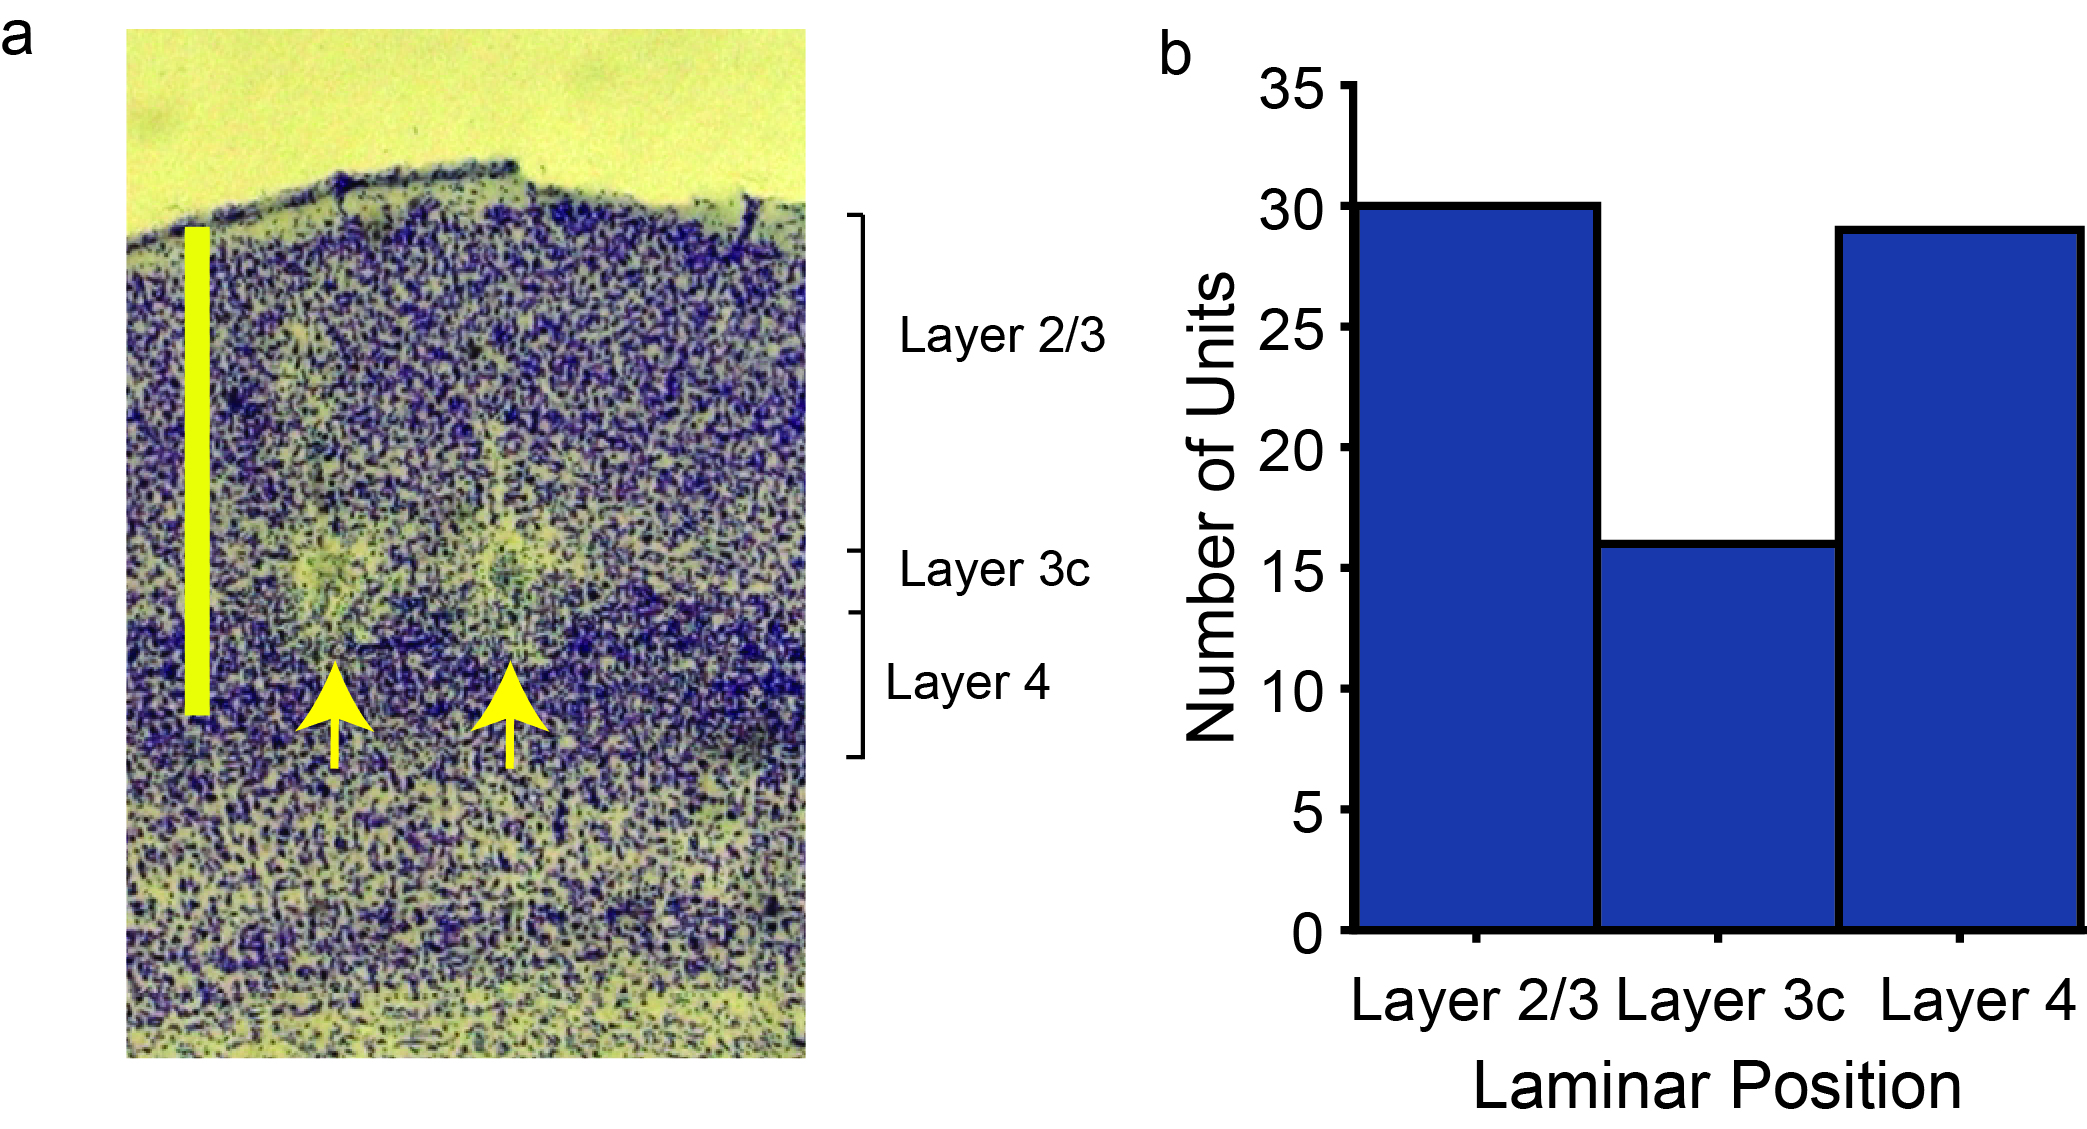
\includegraphics[width=\linewidth]{ShrewV1/LaminarPosition.jpg}
	\caption{The distribution of laminar positions from which we recorded. a) A photomicrograph of the tree shrew primary visual cortex with layers 2/3, 3c and 4 marked. The two arrows point to two lesions made in layer 3c of two separate tracks. The scale bar is 1 mm. b) Histogram showing the number of neurons recorded from each of the layers.}
	\label{fig:lp}
\end{figure} 

\subsubsection{Distribution of the circular variance}

The distribution of circular variances for neurons in the three layers, calculated from their responses to thin moving bars are shown in fig \ref{fig:cv}. The median CV of layer 2/3 neurons was 0.59 (n=28; 95\% CI= [0.32, 0.68]) ; that of layer 3c was  0.87 (n= 16; 95\% CI=[0.68, 0.91]) and that of layer 4 was 0.88 (n=29; 95\% CI=[0.84, 0.90 ]). The three distributions were significantly different from each other (p$<$0.001, Kruskal-Wallis test). Post-hoc tests revealed that there was a statistically significant distribution between the distribution of CVs of neurons in layer 2/3 and layer 3c (Mann-Whitney U test, z=2.37; p$<$0.01) and between layer 2/3 and layer 4 (Mann-Whitney U test, z= 3.58, p$<$0.001). The difference between the distributions of CV of layer 3c neurons and layer 4 neurons was not statistically significant (Mann-Whitney U test, z= 0.67; p=0.25). 
	\begin{figure}[H]
	
	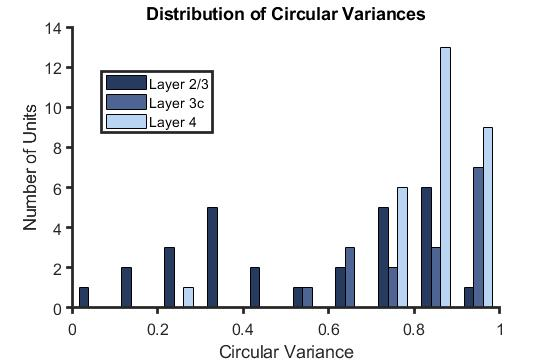
\includegraphics[width=\linewidth]{ShrewV1/cv_lamina_2_bw.jpg}
	\caption{The distribution of circular variance of neurons of the shrew V1.}
	\label{fig:cv}
\end{figure} 

\subsubsection{Circular mean of neurons}

According to our scheme of orientation selectivity in the tree shrews, layer 2/3 neurons inherit their orientation selectivity from layer 4 neurons which are biased for orientation. Here we test this hypothesis. Further, neurons in the tree shrew Layer 4 were thought to be untuned to orientation. However, recent studies, along with our own results in fig \ref{fig:cv} show that these neurons show orientation biases. Hence, we also wanted to determine if the orientation columns reported in the shrew Layer 2/3 extended to layer 4. As a result, we took the absolute difference between the circular means of each layer 2/3 neurons and subsequent neurons recorded from layers 3c and 4. These are shown in fig \ref{fig:cmdiff}.
	\begin{figure}[H]
	
	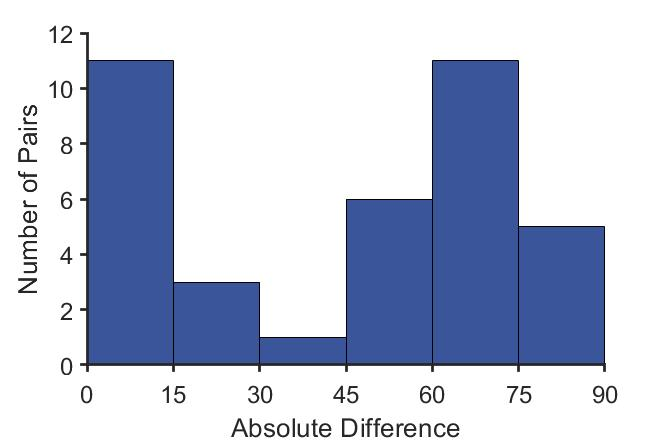
\includegraphics[width=\linewidth]{ShrewV1/cmdiff.jpg}
	\caption{The absolute difference between the circular mean of the first layer 2/3 neurons in each track and subsequent neurons from layer 3c and layer 4 in each track.}
	\label{fig:cmdiff}
	\end{figure}

Instead of the expected unimodal distribution where most neurons in a track were tuned to the same orientation, our results showed a bimodal distribution with approximately half the neurons tuned to the same orientation as the layer 2/3 neuron while the other half was tuned to an orientation that was 65$^o$ away.

We then split the distribution in two groups: pairs of neurons that were tuned to orientations less that 45$^o$ (group 1) apart and pairs tuned to orientation greater than 45$^o$ apart (Group 2). We then looked at whether the difference of was between the layer 2/3 neuron and layer 3c neurons or between layer 2/3 neuron and layer 4 neurons. These results are shown in fig \ref{fig:cmlayer}. We found that in group 1, the majority of the difference pairs were between layer 2/3 and layer 4 neurons (N=15; Binomial Distribution, p=0.04). In group 2, majority of the difference pairs were between layer 2/3 and layer 3c neurons (N=22; Binomial Distribution, p=0.04)

	\begin{figure}[H]
		
		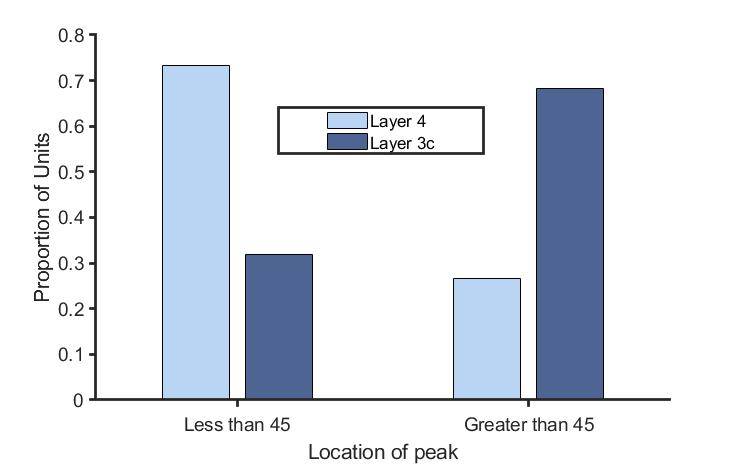
\includegraphics[width=\linewidth]{ShrewV1/cmlayer.jpg}
		\caption{The proportion of neurons from layers 3c and layer 4 with absolute differences greater and lesser than 45$^o$.}
		\label{fig:cmlayer}
	\end{figure}

In order to ensure that the second peak we observed in fig \ref{fig:cmdiff} wasn't due to track angles, we undertook a simulation experiment (see Methods, Random Simulation). We found that for the shortest distance between the layer 2/3 and layer 4 neurons in our sample (50 mm), there was a high probability of getting an absolute difference of 0 but this probability decreased steadily. For the greatest distance in our sample (300 mm), the probability of obtaining the same orientation diminished significantly. While there was a general trend towards getting neurons that were tuned 90$^o$ apart but there was no specific bias for a difference of 65$^o$. The highest probability of obtaining a peak at 65$^o$ was when distance was set at 250 mm (p=0.045).
		\begin{figure}[H]
		
		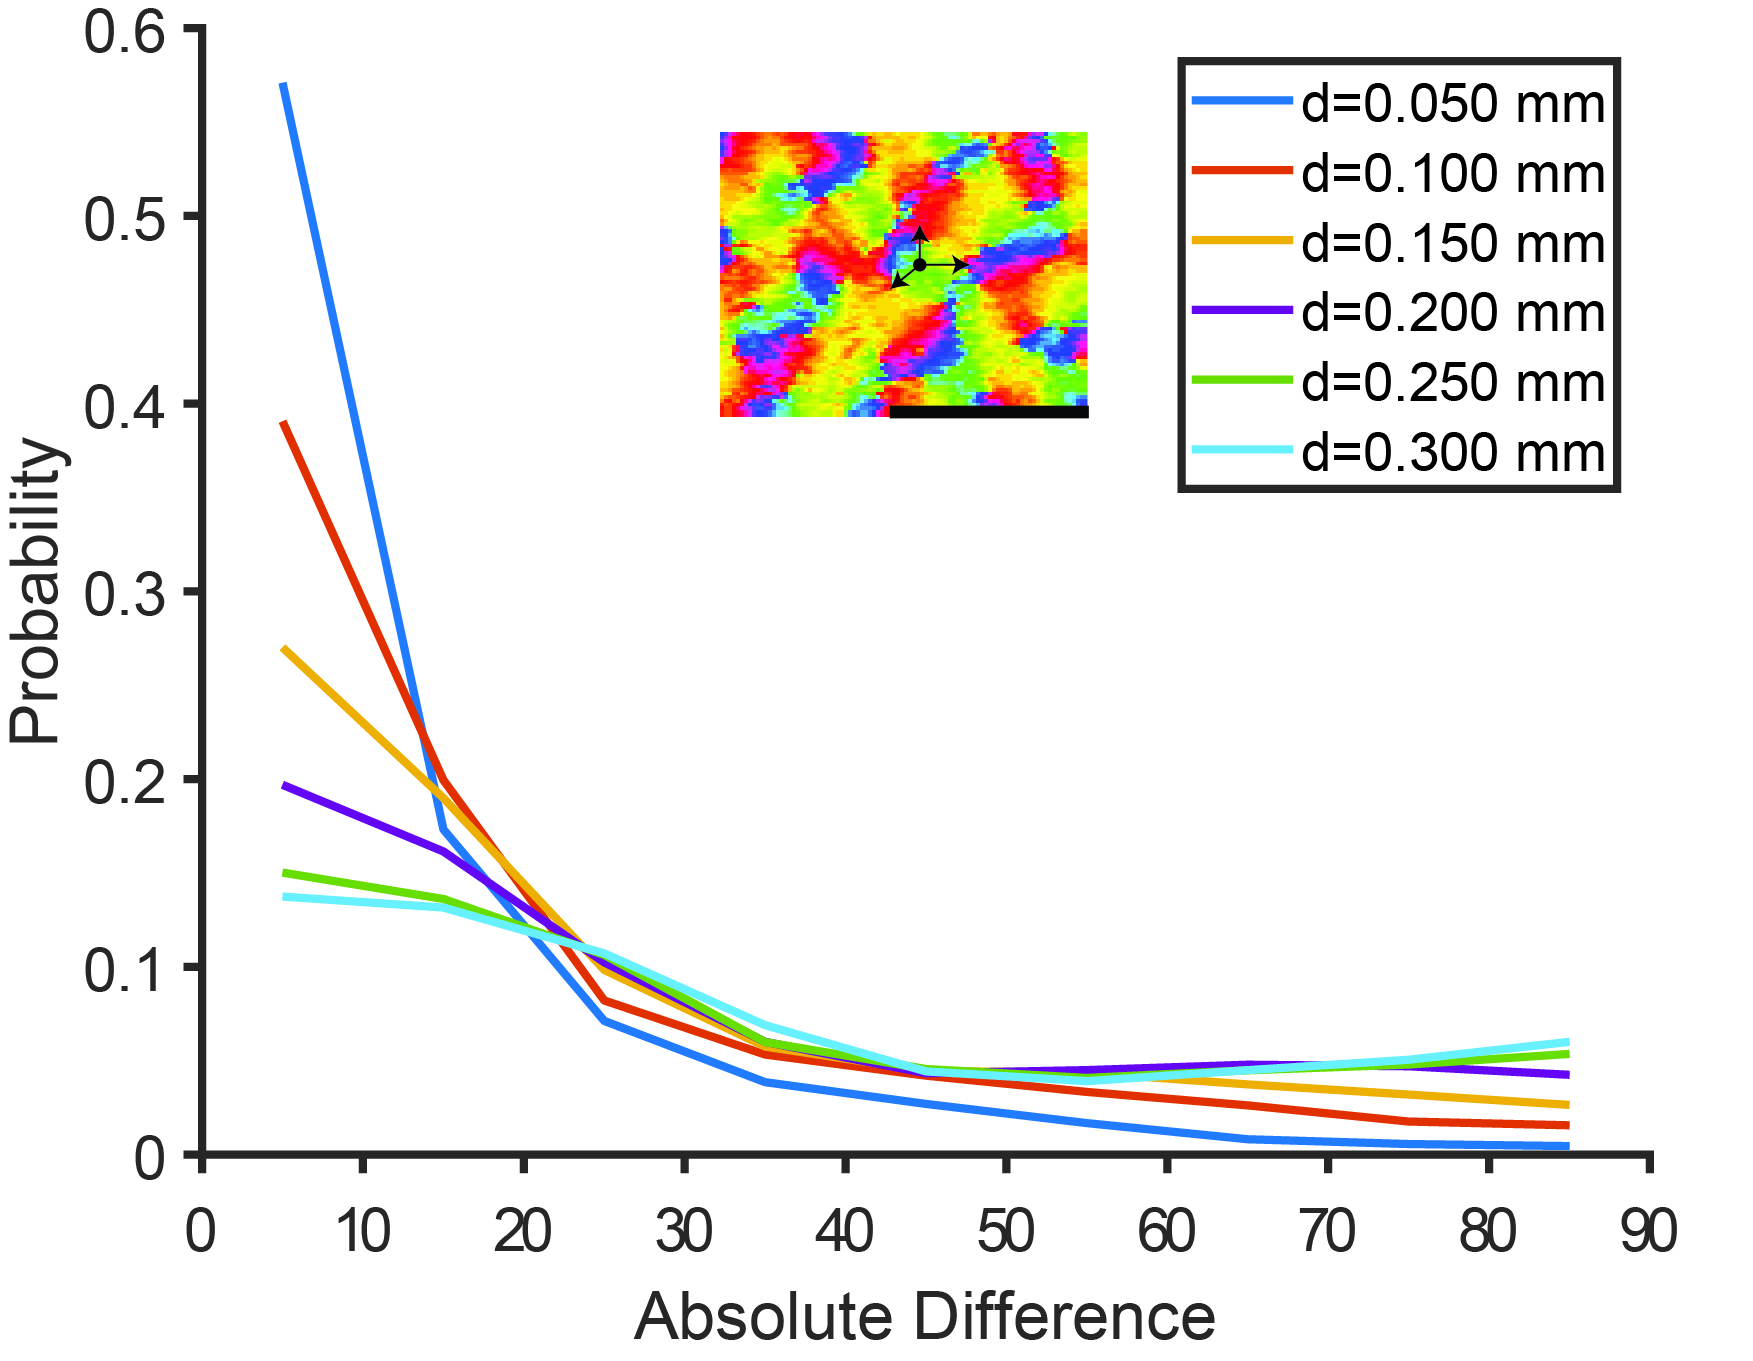
\includegraphics[width=\linewidth]{ShrewV1/simulation.jpg}
		\caption{Results of a simulation experiment: The orientation tuning map (inset) was taken from Bosking et al., 1997. On this map, points were randomly placed and the orientation of 1000 pixels randomly selected at one of the distances in the legend was subtracted from the original data point. For each distance, the distribution of absolute differences for the 1000 pixels are shown by the lines in the graph. Black line is 1mm.}
		\label{fig:sim}
	\end{figure}

\subsubsection{Spatial Frequency Tuning of neurons}

The distribution of the low cut-off, preferred and high cut-off spatial frequencies of the neurons in layer 2/3 and layer 4are shown in fig \ref{fig:sftuning}. Results from only these two layers are shown as we propose that the orientation selectivity of layer 2/3 neurons arise predominantly from layer 4 neurons. We found no significant differences between the spatial frequency tuning between the two layers, although layer 2/3 neurons show high spatial frequency attenuation. When the bandwidth of spatial frequency tuning in octaves was calculated, we found that the layer 2/3 neurons showed slightly sharper tuning (Median layer 2/3 b$_{oct}$= 2.2; n=16; Median layer 4 b$_{oct}$=2.3; n=9). This difference was however not statistically significant (Mann-Whitney U test; z=-1.18; p=0.24).

		\begin{figure}[H]
		
		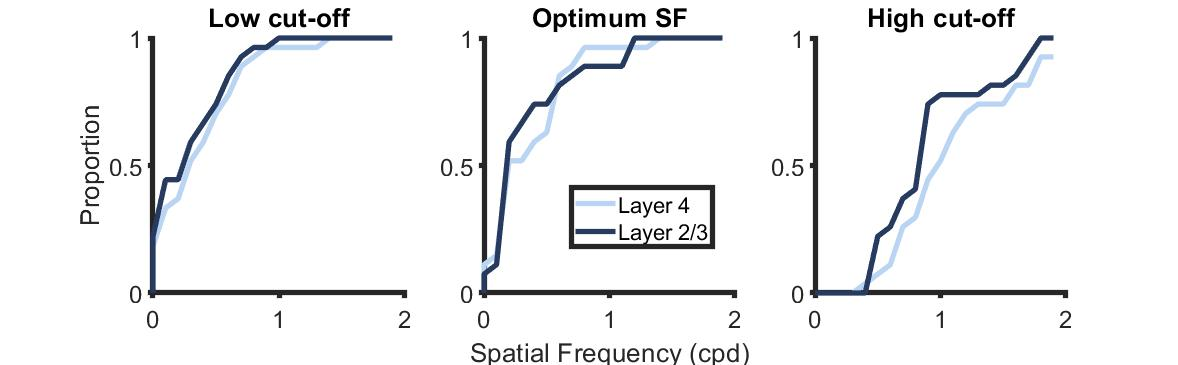
\includegraphics[width=\linewidth]{ShrewV1/sftuning_neurons_2.jpg}
		\caption{The cumulative distribution of the spatial frequency tuning of neurons in layers 2/3, 3c and 4 of the Shrew V1.}
		\label{fig:sftuning}
	\end{figure}

In 18 individual tracks, we compared the spatial frequency and orientation tuning of the layer 2/3 neuron to that of the first layer 4 neuron we encountered. The results of this analysis is shown in fig \ref{fig:sfsum}. The result from an example neuron is shown in parts a and b. Fig \ref{fig:sfsum}a shows that spatial frequency tuning curve of layer 2/3 neuron and that of the layer 4 neuron to optimum and orthogonal orientation. We expected that the optimum spatial frequency of the layer 2/3 neuron and the spatial frequency at which the layer 4 neurons was most tuned for orientation would be similar. We found that this relation held true only in 3 of our 18 tracks. In most of the tracks the maximum OSI of the layer 4 neuron occured at much higher spatial frequencies when compared to the optimum spatial frequency of the layer 2/3 neuron as demonstrated by the data points skewed closer to the y-axis.
	\begin{figure}[H]
	
		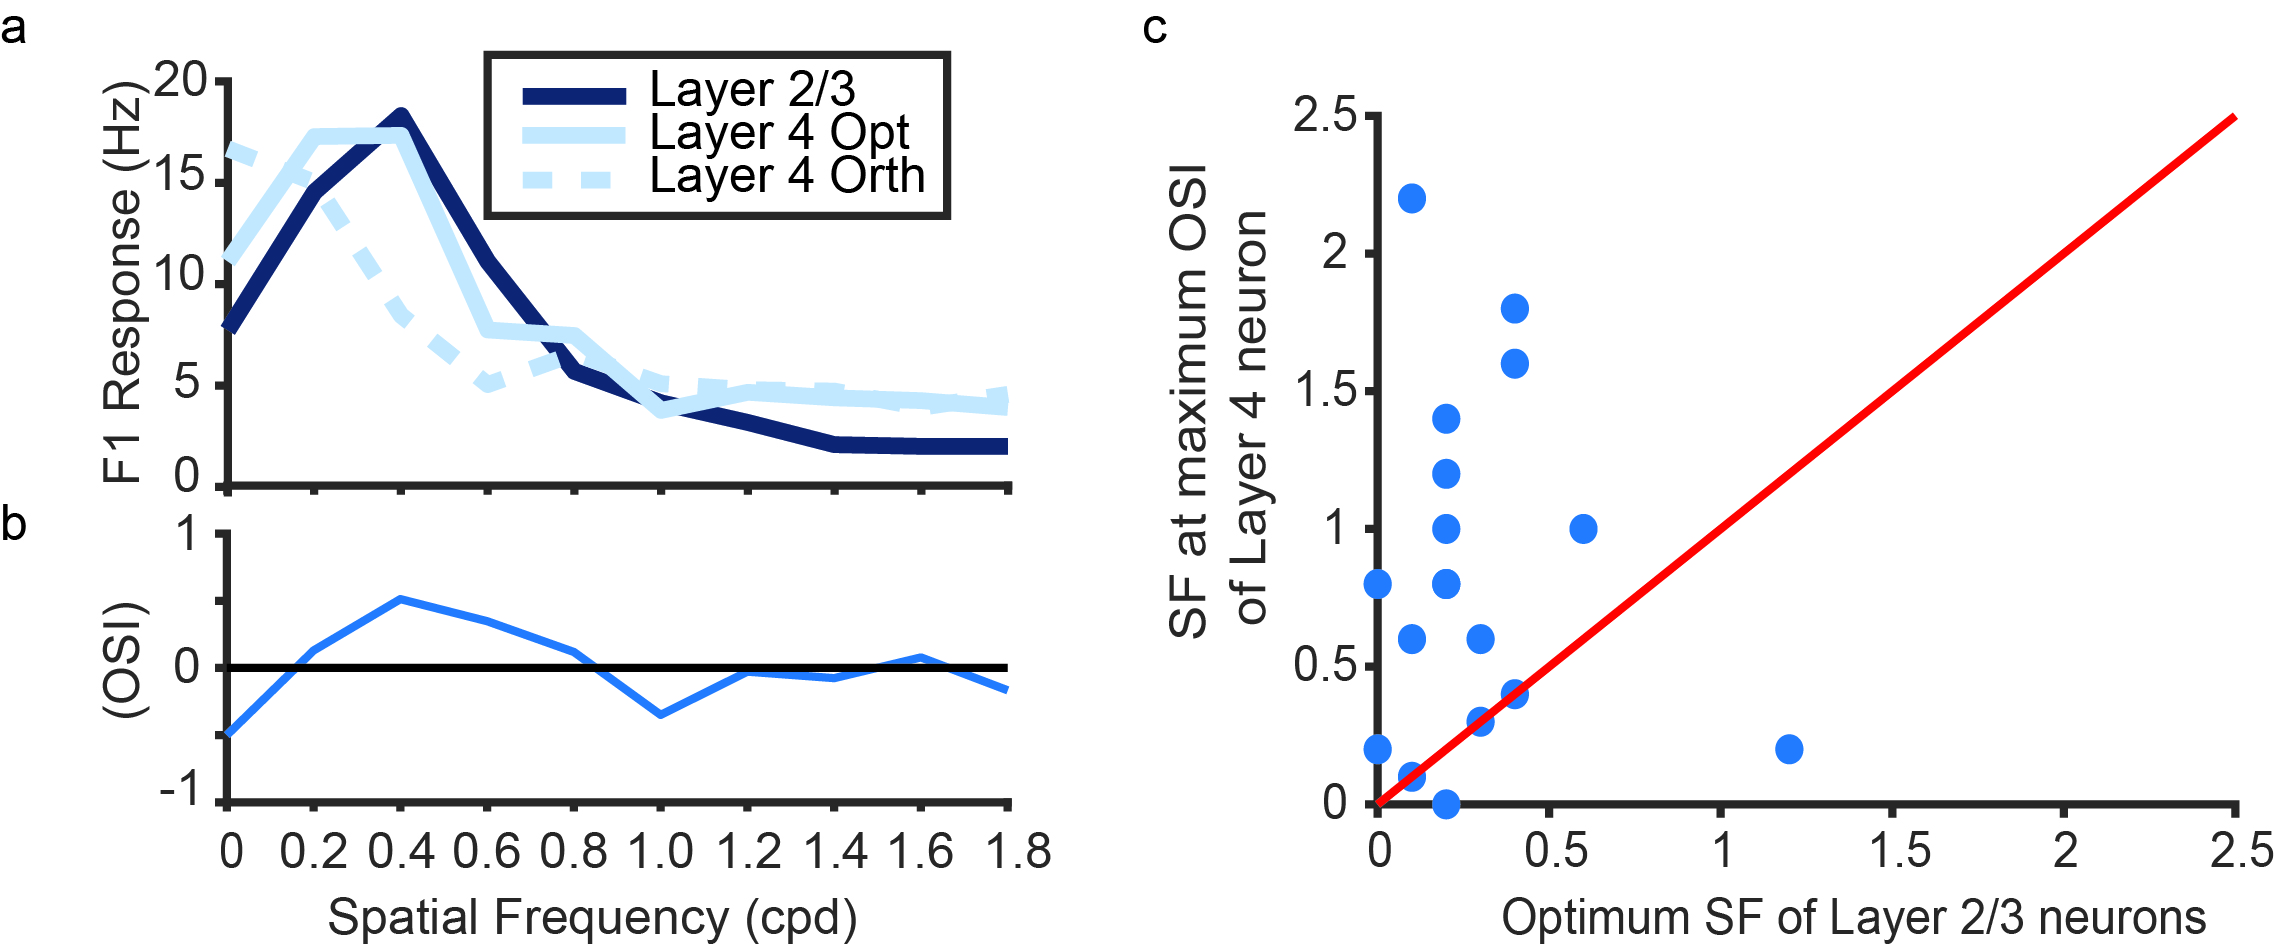
\includegraphics[width=\linewidth]{ShrewV1/sfsummary.jpg}
		\caption{The cumulative distribution of the spatial frequency tuning of neurons in layers 2/3, 3c and 4 of the Shrew V1.}
		\label{fig:sfsum}
	\end{figure}

\section{Discussion}

In this chapter we set out to test if the orientation tuning of layer 2/3 neurons in the tree shrew primary visual cortex could arise by the sharpening of orientation biased inputs from layer 4 using non-specific inhibition. As we hypothesised, the orientation selectivity of the layer 4 neurons sharpened at higher spatial frequencies. We also found that the orientation selectivity of the layer 4 neuron and the corresponding layer 2/3 neurons were similar, however, the neurons in layer 3c of the same track seemed to be tuned to an orientation ~65$^o$ away. Finally, we hypothesised that the layer 2/3 neuron's peak sf would be similar to the spatial frequency where the layer 4 neuron showed maximum orientation tuning. We found that this was only true in a small proportion of the neuron pairs in our sample. In a majority of the pairs, the layer 4 neuron was optimally tuned at spatial frequencies higher than the optimum spatial frequency of the neurons. These results are further discussed below.


\paragraph{Distribution of orientation selectivity}

In this chapter we determined the orientation selectivity using bars for 73 V1 neurons from Layers 2/3, 3c and 4. We found that most neurons in layer 4 and layer 3c were broadly tuned for orientation. The broad orientation selectivity measured in the layer 4 is also consistent with this layer being similar to the LGN neurons when it comes to orientation selectivity (Reference). Layer 2/3 neurons show a bimodal distribution of orientation tuning when tested using bars with one group of neurons tuned quite sharply to orientation and another group tuned fairly broadly to orientation. There were no further sub-laminar differences in the distribution of this orientation selectivity within layer 2/3. These results are consistent with those reported earlier in the tree shrews (Van Hooser et al., 2013). 

Our results in layers 2/3 of the tree shrews are also consistent with those reported earlier in cats and macaques, where neurons in the primary visual cortex show a wide variety of orientation selectivities regardless of the layer. It should however be noted that neurons in layer 4 of the cats already show fairly sharp orientation selectivity and in layer 4C$\alpha$ of macaques too there are neurons that show sharp orientation selectivity. However neurons in layer 4C$\beta$ show broad orientation selectivity and regardless of the median orientation selectivity, neurons in all layers showed a wide range of orientation selectivity, especially as reported in layer 2/3 here (Ringach et al., 2002 etc).

\paragraph{Orientation selectivity of layer 3c neurons}

In our sample, we found that the neurons of layer 3c in the shrew V1 were broadly tuned to orientation despite being in the supragranular layers. These results are similar to those reported by Van Hooser and colleagues. In an earlier paper, it was shown that neurons in top and bottom parts of layer 4 projected to layer 3c (Fitzpatrick, 1996). The layer 4 neurons that project to the layer 3c neurons show sharper orientation tuning when compared to that of the layer 3c neurons. However, it makes no sense to develop orientation selectivity only to loose it at the very next step of processing. An alternate explanation could be that the broad orientation selectivity we see in the layer 3c is due to neurons in this layer receiving direct LGN inputs from layer 2(?), which is meant to have W-like cells. Similarly the layer 3C analogue in the macaques, layer 3B neurons which receive strong koniocellular inputs also show broad orientation tuning.

Another possibility could be that the neurons in layer 3c could be providing inhibitory inputs to the layer 2/3 neurons. The optimum orientation of the neuron was often 65$^o$ away from the orientation of the layer 2/3 neuron. In our scheme, layer 2/3 neurons sharpen the orientation biases from the layer 4 neurons by disynaptic inhibitory inputs from neurons tuned to orthogonal orientations. Anatomically, these inputs could be provided by the extensive horizontal connections in layer 2/3. However, having neurons tuned to the orthogonal or near orthogonal orientation organised in layers could provide an economy of connections that the long range horizontal inputs could not provide. In line with this, it has been shown that layer 3c does not have any significant horizontal connections and project upwards into layer 2/3, indicating that these neurons could be the source of the unoriented or orthogonally oriented disynaptic inhibitory inputs.

\paragraph {Spatial Frequency Dependence of Orientation Tuning in layer 4 neurons}

When we examined to see if the orientation selectivity of layer 4 neurons varied in relation to the spatial frequency tuning of the neurons, we found that in most cases, layer 4 neurons showed sharper orientation selectivity at higher spatial frequencies. This sharpening at high spatial frequencies has been previously reported in the retina and LGN of cats (Hammond, 1974; Levick and Thibos, 1980, 1982; Vidyasagar and Urbas, 1982) and macaques (Passaglia et al., 2002; Smith et al., 1990). This indicates that the sharpening of orientation selectivity observed from the layer 4 to layer 2/3 neurons in this case might employ a similar mechanism to that in cats---from LGN to layer 4--- and in macaques --- from Magnocellular layers in LGN to layer 4C$\alpha$. We also found that in some cases, the orientation selectivity of the neuron was higher at lower spatial frequencies. We are unsure what this is about.


\paragraph{Distribution of Spatial Frequency}

We examined the difference in the spatial frequency tuning between layer 2/3 neurons and layer 4 neurons. According to our scheme, if layer 2/3 neurons got their orientation selectivity from layer 4 neurons, then, a higher proportion of layer 2/3 neurons will show bandpass spatial frequency tuning when compared to layer 4 neurons. However, we found that there was no significant difference in the proportion of band pass tuned neurons between layer 4 and layer 2/3. These results are contradictory to those reported in by Van Hooser et al., 2013. One sigificant difference between our studies is the method used to estimate the spatial frequency tuning. They used a difference of gaussian curve to get the low cut-off, peak and high-cutoff spatial frequencies of the neurons. This method assumes that neurons have center-surround organisation as has been shown in the retinal ganglion and LGN neurons. Mathematically, they also did not use a separate term for the peak spatial frequency which means that the fit would only show a band-pass spatial frequency tuning if the peak spatial frequency was significantly greater than 0 cpd. We found that a significant proportion of neurons in our sample had fairly low optimum spatial frequencies which  may have been classified as low pass tuning using the DOG method whereas were classified as band-pass tuned using our method. We also found that there was a small degree of high spatial frequency attenuation in the neurons. This could be due to the small increase in receptive field sizes from layer 4 to layer 2/3 which reduces acuity. This high spatial frequency attenuation also explains the narrower tuning bandwidths of layer 2/3 neurons.

We also hypothesised that the peak spatial frequency of the layer 2/3 neurons would be similar to the spatial frequency where the orientation tuning of the layer 4 neuron was greatest. However, we found this in only a small proportion of the neurons in our study. For this to be the case in a majority of the studies, layer 2/3 neurons needed to have higher peak spatial frequencies when compared to the layer 4 neurons. However, there hasn't been any systematic overrepresentation of higher spatial frequencies in the layer 2/3 neurons in our study. Several studies in the past have suggested that neurons in the V1 of cats and macaques may be organised in columns, similar to that seen in orientation selectivity. We didn't find any such consistency either. There seems to be a continuous distribution of most spatial frequencies in the cortex. As a result, within a single track, there could be several neurons all tuned to different spatial frequencies projecting the layer 2/3 neurons. As a result, for this hypothesis to be tested correctly, we would need to undertake simultaneous recordings from the layer 2/3 and layer 4 neurons and record from pairs that are connected. Despite these caveats, we found our expected results in 3 pairs of neurons with a few other pairs bunched close to the identity line. As a result, while we cannot definitely conclude that neurons in layer 2/3 use non-specific inhibition to sharpen the orientation biases inherited from the layer 4 neurons, we do have some evidence that suggests that this could be the mechanism through which orientation arises in some neurons in the tree shrew V1. 

